\documentclass[crop,tikz]{standalone}

\usepackage{fontspec}
\setmainfont{texgyrepagella}[
  Extension = .otf,
  UprightFont = *-regular,
  BoldFont = *-bold,
  ItalicFont = *-italic,
  BoldItalicFont = *-bolditalic,
]

\usepackage{tikz}
\usetikzlibrary{decorations.pathreplacing,calligraphy}
\usetikzlibrary{calc}

\makeatletter % https://tex.stackexchange.com/a/38995/121799
\tikzset{
  use path/.code={\pgfsyssoftpath@setcurrentpath{#1}}
}
\makeatother
\tikzset{reverseclip/.style={insert path={(current bounding box.north
        east) rectangle (current bounding box.south west)}}}

\pgfdeclarelayer{bg}
\pgfsetlayers{bg,main}


\begin{document}

\pgfdeclarelayer{img}
\pgfsetlayers{img,bg,main}

\begin{tikzpicture}
    \begin{pgfonlayer}{img}
        \node[anchor=south west,inner sep=0] (image) at (0,0) {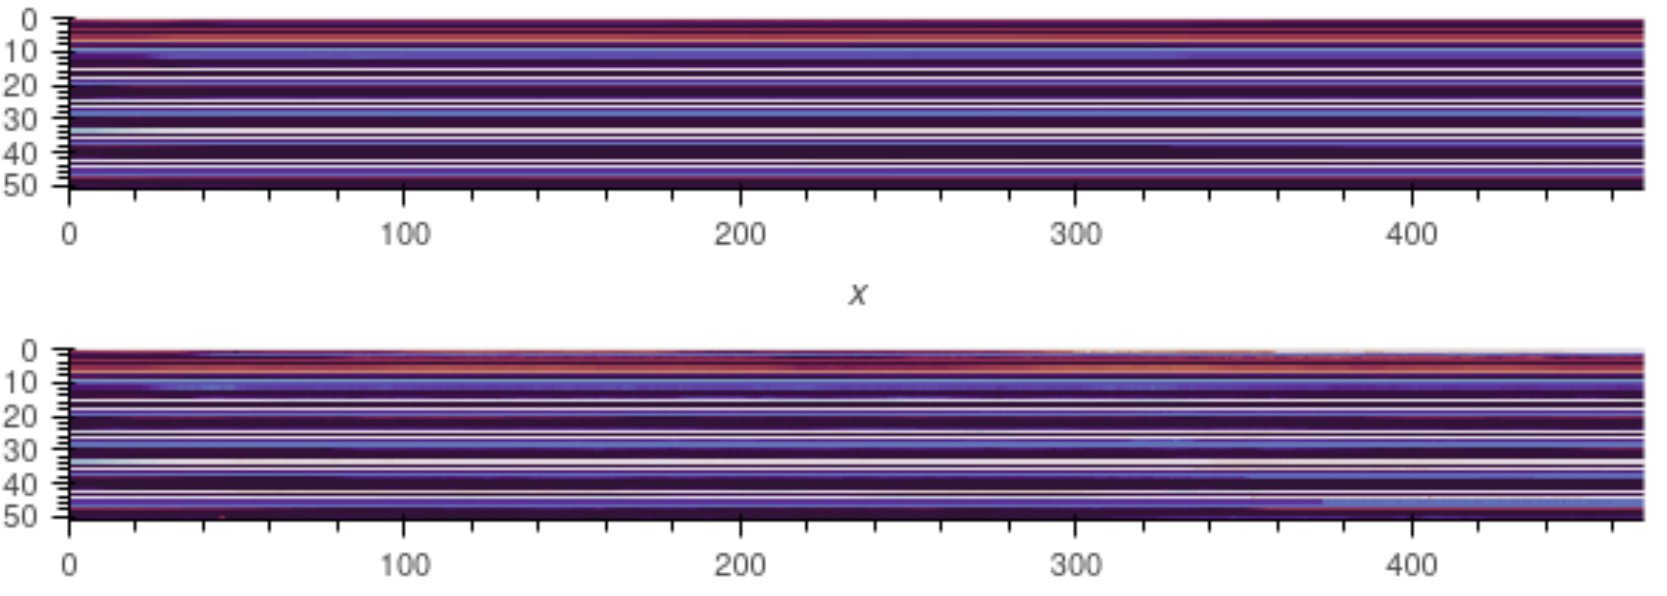
\includegraphics[width=15cm]{probabilistic-model-predictions.png}};
    \end{pgfonlayer}
    \begin{scope}[x={(image.south east)},y={(image.north west)}]
        \draw[thick,decorate,decoration={calligraphic brace,raise=5pt, amplitude=5pt}] (-0.01, 0.68) -- node[anchor=south,left=10pt] {Target Angles} (-0.01, 0.98);
        \draw[thick,decorate,decoration={calligraphic brace,raise=5pt, amplitude=5pt}] (-0.01, 0.12) -- node[anchor=south,left=10pt] {Predicted Angles} (-0.01, 0.44);
        \draw[thick,decorate,decoration={calligraphic brace,raise=5pt, amplitude=5pt}] (0.99, -0.08) -- node[below=10pt] {Time} (0.03, -0.08);
        \draw[thick,decorate,decoration={calligraphic brace,raise=-5pt, amplitude=5pt}] (0.04, 0.48) -- node[above=5pt] {} (0.12, 0.48);
        \draw[thick,decorate,decoration={calligraphic brace,raise=5pt, amplitude=5pt}] (0.12, 0.06) -- node[below=10pt] {30 Seed Frames} (0.04, 0.06);
        \draw[->] (0.08, 0.68) -- (0.08, 0.485);
    \end{scope}
\end{tikzpicture}

\end{document}
